\documentclass{standalone}
\usepackage{mathpazo}
\usepackage{siunitx}
\usepackage[american voltages, american currents, american inductors]{circuitikz}
\usetikzlibrary{calc}
\newcommand*{\equal}{=}

\begin{document}
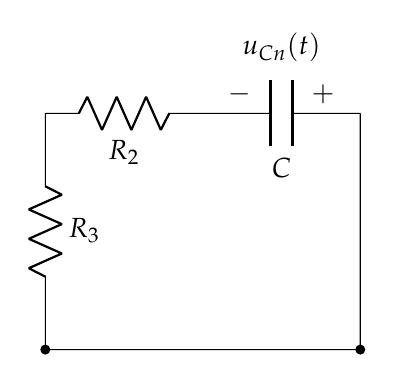
\begin{tikzpicture}
  \draw
  (0,0) to [C, l = $C$, v=$u_{Cn}(t)$] ++(-2, 0) 
  to [R, l = $R_2$] ++(-2, 0) 
  to [R, l = $R_3$] ++(0, -3)
  (0,0) to [short] ++(0,-3)
  to [short, *-*] ++(-4,0);
  \end{tikzpicture}
\end{document}